\documentclass[11pt]{article}

\usepackage[activate={true,nocompatibility},final,tracking=true,kerning=true,spacing=true,factor=1100,stretch=10,shrink=10]{microtype}
\usepackage{multirow}
\usepackage{mathtools}
\usepackage{graphicx}
\usepackage{tabularx}
\usepackage{enumerate}
\usepackage{amsmath, amssymb, graphics, setspace}
\usepackage[noline,noend,ruled,linesnumbered]{algorithm2e}
\usepackage{algpseudocode}
\usepackage{enumitem}
\usepackage{amssymb}
\usepackage{amsmath}
\usepackage{latexsym}
\usepackage{graphics}
\usepackage{multirow}
\usepackage{verbatim}
\usepackage[T1]{fontenc}
\usepackage{subfigure}
\usepackage{tikz}
\usetikzlibrary{arrows}
\usepackage{url}
\usepackage[noline,noend,ruled,linesnumbered]{algorithm2e}
\usepackage{algpseudocode}

\DeclareMathOperator{\lcm}{lcm}

\newcommand{\mathsym}[1]{{}}
\newcommand{\unicode}[1]{{}}

\title{Assignment 3}

\author{Paul Jones and Matthew Klein \\
		Professor Kostas Bekris\\
		Design and Analysis of Computer Algorithms (01.198.344)}

\date{\today}

\usepackage{setspace}
\singlespacing
 \usepackage{url} 
\usepackage[letterpaper]{geometry}
\geometry{top=1in, bottom=1in, left=.5in, right=.5in}

\usepackage{fancyhdr}
\pagestyle{fancy}
\lhead{Paul Jones and Matthew Klein \\ Professor Kostas Bekris}
\chead{}
\rhead{Design and Analysis of Computer Algorithms \\ Rutgers University}
\lfoot{}
\cfoot{\thepage}
\rfoot{}

\begin{document}

\subsection*{Problem 1} After the departure of Storm
Sandy, the small town of New Town suffered an electricity power
shortage. After this experience, the local electricity agent decided
to create plans to better handle future events. The idea is to send
out immediately after the power failure a truck to investigate the
damage along every street in the town. In order to recover the
electricity network as soon as possible, they want to find an
efficient tour so that the truck visits each street exactly once and
then goes back to the town headquarters. Suppose each street in New
Town is a two-way street. The task is to find whether there exists a
tour that visits each street only once and then goes back to the
starting point.\\

\begin{enumerate}[label=\textbf{\Alph*.}]
\item  \textbf{Show that the problem has a solution if and only if
there are no dead ends and no $n$-way junctions in New Town, where $n$
is odd, i.e., each intersection in the town has an even degree.}

Since each intersection has an even degree, there is definitely a solution as this is an Euler Tour. Dead ends are also odd junctions, as $n = 1$. Start with any vertex, or town, and repeatedly go to a street that doesn't separate the entire graph. Once we find a street that separates the graph, we are done. Until then we add the street, then remove it (so we don't visit it again) and repeat. If we end up separating the graph by going to a wrong street, we will not be able to visit that section of New Town.

\item  \textbf{If such tour exists, please describe an efficient
algorithm to find the tour in linear time, i.e., in at most $O(|V| +
|E|)$ time, where $V$ is the set of junctions and $E$ is the set of
streets.}

We can do the algorithm stated previously:

Start with any vertex, or town, and repeatedly go to a street that doesn't separate the entire graph. Once we find a street that separates the graph, we are done. Until then we add the street, then remove it (so we don't visit it again) and repeat. If we end up separating the graph by going to a wrong street, we will not be able to visit that section of New Town.

This is $O(|V| + |E|)$ time, as we at most visit every single street once and every single town once. Everything that separates the graph is saved for the end. So, we go down a street and lower our $|E|$ by one, and then go to another $|V|$. We repeat going down the $|E|-i$ streets, and the $|V|-i$ junctions until none remain. As we only take one street or junction each time, the running time is $O(|V| + |E|)$.

\end{enumerate}


\subsection*{Problem 2: [25 points]} In a chemistry class, the
professor asks you to synthesize products using existing
chemicals. For instance, 2 parts of chemical A produces 1 part of
chemical B, or 3 parts of chemical C can give us 1 part of chemical
D. Lets assume that we have $n$ different chemicals that we can
mix. The production ratio given two chemicals is fixed and does not
change. These ratios are given in an $n \times n$ matrix, between all
the chemicals. In particular, using $x$ parts of chemical $i$ you will
receive $R_{ij} \cdot x$ parts of chemical $j$, or using $y$ parts of
chemical $j$ you will receive $R_{ji} \cdot y$ parts of chemical
$i$. Note that $R_{ij}$ is not necessarily an integer, it can be a
real number.\\

\noindent Because of the principle of mass conservation the ratios
have to satisfy the following requirement: $R_{ij} \cdot R_{ji} <
1$. This means that converting an amount of chemical $i$ to chemical
$j$ and then back to chemical $i$ should result in a smaller quantity
of chemical $i$ relatively to the original one.\\

\begin{enumerate}[label=\textbf{\Alph*.}]
\item  \textbf{The Chemistry professor asks from you the
following. Given the $n \times n$ matrix, find the best sequence of
chemical reactions to produce the most of chemical $D$ given an
available quantity of chemical $A$. As mentioned before there are $n$
different chemicals you can use and the matrix specifies the
production ratios of all corresponding reactions. Provide an algorithm
for finding the best sequence. Argue about the running time of your
algorithm.}

First, I will cover what data structure will best represent this
graph. Then, I will cover the best algorithm to solve the problem
given my choice of data structure.

Notice the structure of the matrix and how it can be represented
as a graph where we can exploit certain properties to find the 
answer we are after. First, our $n \times n$ matrix can be represented
as a graph in the following way. Each cell $R_{ij}$ can be a node
representing a specific chemical with edges between it and every
other chemical node where the edges represent the conversion factor
for production. It \emph{does} have an edge to itself, with value
of $1$ necessarily, because if you have chemical $A$ and you want
to produce chemical $A$ you needn't do any steps and you retrieve
all of your chemical.

The graph I'm advancing is one where every chemical
is a node, and every conversion ratio is an edge weight. The value
of the edge weight will be the underlying fraction of the ratio,
where if the ratio is $1 : 2$, the weight will be $0.5$, if the
ratio is $1 : 3$, the weight will be $.3$ repeating, and if the
ratio is $3 : 5$, the weight will be $.6$, etc.

Here is a graphical representation of
chemicals $A$ through $D$ with various production ratios simplified
to fractions:

\begin{center}
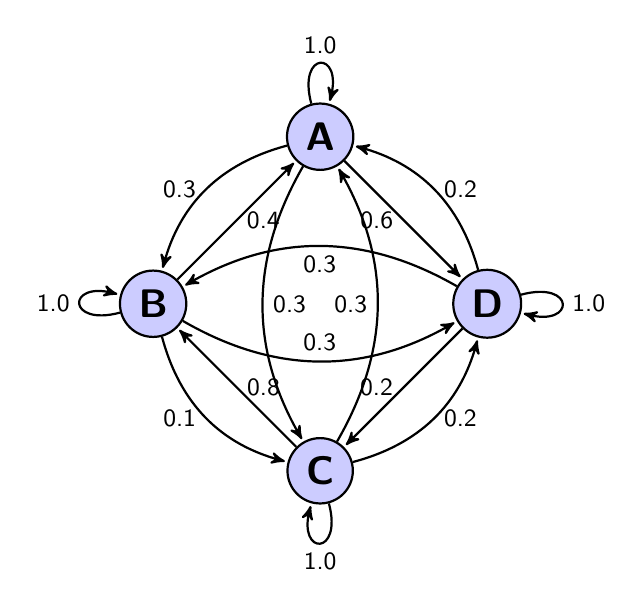
\begin{tikzpicture}[->,>=stealth',shorten >=1pt,auto,node distance=3cm,
  thick,main node/.style={circle,fill=blue!20,draw,font=\sffamily\Large\bfseries}]

  \node[main node] (1) {A};
  \node[main node] (2) [below left of=1] {B};
  \node[main node] (3) [below right of=2] {C};
  \node[main node] (4) [below right of=1] {D};

  \path[every node/.style={font=\sffamily\small}]
    (1) edge node [left] {0.6} (4)
        edge [bend right] node[left] {0.3} (2)
        edge [bend right] node {0.3} (3)
        edge [loop above] node {1.0} (1)
    (2) edge node [right] {0.4} (1)
        edge [bend right]node {0.3} (4)
        edge [loop left] node {1.0} (2)
        edge [bend right] node[left] {0.1} (3)
    (3) edge node [right] {0.8} (2)
        edge [loop below] node {1.0} (4)
        edge [bend right] node {0.3} (1)
        edge [bend right] node[right] {0.2} (4)
    (4) edge node [left] {0.2} (3)
        edge [loop right] node {1.0} (4)
        edge [bend right] node {0.3} (2)
        edge [bend right] node[right] {0.2} (1);
\end{tikzpicture}
\end{center}

What structure should be used to store this graph? Well, we're
coming from a matrix where I characterized the value in $R_{ij}$
as the edge weights in a graph where the $i$th chemical to the
$j$th chemical is the node, so it is going to be very dense.
The best way to store dense graphs is an adjacency matrix.
This makes look-up very fast as well, which will be important to
us.

Now that I've covered my data structure, I'm going to cover
the algorithm I use to solve the problem as characterized
as a graph problem.
The chemist is asking for the path on the graph with the highest
value if the cost of the path is the value of every edges weight
multiplied. That is, if you were going from $A$ to $B$ to $C$ to $D$, 
the cost would be $.3 \times .1 \times .2$. This would be a very
bad return value, admittedly, specifically it would yield a return
at $.006$. We want \emph{the highest value} end multiple with a \emph{single
source} and a \emph{single destination}.

There will be $n$ nodes and $n^2$ edges, because every node has an edge
to every node including itself. And the solution that
the chemist wants is the path where the product all the edges between
the chemical we \emph{have} and the chemical we \emph{want} is the
\emph{highest}. The best algorithm to solve the single-pair shortest
path algorithm is the A* algorithm, but we'll have to make a change
to suit our needs.

The A* algorithm is Dijkstra's algorithm with the addition of best-path
and heuristics. 
From the book \emph{Artificial Intelligence: A New Synthesis}:

\begin{enumerate}[label={\arabic*.}]
\item Create a search graph $G$, consisting solely of the start node, $n_o$. Put $n_o$ on a list called OPEN.
\item Create a list called CLOSED that is initially empty.
\item If OPEN is empty, exit with failure.
\item Select the first node on OPEN, remove it from OPEN, and put it on CLOSED. Called this node $n$.
\item If $n$ is a goal node, exit successfully with the solution obtained by tracing a path along the pointers from $n$ to $n_o$ in $G$. (The pointers define a search tree and are established in Step 7.)
\item Expand node $n$, generating the set $M$, of its successors that are not already ancestors of $n$ in $G$. Install these members of $M$ as successors of $n$ in G.
\item Establish a pointer to $n$ from each of those members of $M$ that were not already in $G$ (i.e., not already on either OPEN or CLOSED). Add these members of M to OPEN. For each member, $m$, of $M$ that was already on OPEN or CLOSED, redirect its pointer to $n$ if the best path to $m$ found so far is through $n$. For each member of $M$ already on CLOSED, redirect the pointers of each of its descendants in $G$ so that they point backward along the best paths found so far to these descendants.
\item Reorder the list OPEN in order of increasing $f$ values. (Ties among minimal $f$ values are resolved in favor of the deepest node in the search tree.)
\item Go to Step 3.
\end{enumerate}

The modification we need to make for our purposes is to change the
way that distance is computed. In step 5, where ``exit successfully with the solution obtained by tracing a path'', the function used to get the path
will need to do multiplication instead of addition. Furthermore, in step
8 where ``Reorder the list OPEN in order of increasing f values.'', the
values are going to be determined by multiplication and not addition.
The path-cost function will be multiplication of past values for all
uses of the heuristic. The heuristic function that should be used here
is a simple one, where you take the straight conversion from one chemical
into the other to be roughly what it costs to do it, and then compare that
against the actual and various routes. The worst case performance of the
A* algorithm, then, is

$$O(|E|) = O(|V|^2)$$

This is an interesting conclusion because with our sparse graph,
the A* algorithm, which only computes a single-pair shortest path,
will actually yield the same result as Dijkstra's algorithm with
an array implementation, which solves single-source all-pair shortest
path problem. So, for sake of simplicity, I recommend using Dijkstra's
algorithm with an array implementation. The reason you want to use 
an array instead of a binary heap or a Fibonacci heap is because
as the value of $|E|$ approach its maximum of $V^2$, the array implementation
becomes more attractive.

Here is an algorithm description which will solve the problem
given the graph representation I have set up:

\begin{enumerate}[label={\arabic*.}]
\item Assign to every chemical node a tentative cost value: set it to zero for our source node and to infinity for all other chemical nodes.
\item Mark all chemical nodes unvisited. Set the source chemical node as the current node. Create a set of the unvisited chemical nodes called the unvisited set consisting of all the chemical nodes.
\item For the current chemical node, consider all of its unvisited neighbors and calculate their tentative costs, multiplying their fractions together. Compare the newly calculated tentative cost to the current assigned cost and assign the greater one. For example, if the current chemical node A is marked with a cost of $0.6$, and the edge connecting it with a neighbor chemical $B$ has length $0.2$, then the cost of producing to $B$ through $A$ will be $0.6 \times 0.2 = 0.12$. If $B$ was previously marked with a cost greater than than $0.12$ then change it to $0.12$. Otherwise, keep the current value.
\item When we are done considering all of the neighbors of the current chemical node, mark the current chemical node as visited and remove it from the unvisited set. A visited node will never be checked again.
\item If the destination chemical node has been marked visited (when planning a route between two specific nodes) or if the smallest tentative distance among the nodes in the unvisited set is infinity (when planning a complete traversal; occurs when there is no connection between the initial node and remaining unvisited nodes), then stop. The algorithm has finished.
\item Select the unvisited chemical node that is marked with the smallest tentative cost, and set it as the new "current chemical node" then go back to step 3.
\end{enumerate}

This will run a maximum number of times by hitting every $n$ node $n$ times,
because our graph is maximally dense.

$$O(V^2) = O(E)$$

\item  \textbf{One of the teams found out that using chemical
$i_1$ to produce chemical $i_2$, then chemical $i_3$, \dots, then
chemical $i_k$ and back to $i_1$ results in a bigger quantity of
chemical $i_1$ than the original one, i.e., $R_{i_1,i_2} \cdot
R_{i_2,i_3} \cdot \ldots \cdot R_{i_k,i_1} \geq 1$. Is this a problem
in the ratio matrix or the students did something wrong in their
calculations? Provide an efficient algorithm that can detect if such
an impossible sequence of chemical reactions seems feasible given the
$n \times n$ production ratio matrix. Argue about the running time of
your algorithm.}

In the graph representation found above, this would be very easy to
detect. Every edge between two chemicals has a fractional value, and
every duo of chemicals has a conversion to and fro. The only way
to get a value greater than one from a conversion is if the conversion
to another chemical summed with the conversion back from that chemical
is greater than one. For instance, if to convert from chemical $A$ to
chemical $B$, 3 parts $A$ were required for 5 parts $B$, giving that
edge a value of $0.6$. Then, if the matrix also had 2 parts $B$
being required to make $1$ part $A$, resulting in a value on the edge
of $0.5$. Because $0.5 + 0.6 > 1$, the chart and graph contain
values which violate fundamental laws of nature.

The algorithm I'd use to compute this value would begin on chemical 
node $A$ and store the fractional value of the ratio needed to convert
it into every subsequent chemical $B$, $C$, ... When on the opposite
chemical, add to this value the cost of converting back to $A$ from 
$B$, $C$, ... If this value is greater than $1$, then the matrix is
flawed in some way. If not, then the matrix contains no errors \emph{of
this kind}, but may contain others. 

$$O(2n) = O(n)$$

\end{enumerate}

\subsection*{Problem 3: [25 points]} Consider a courier company with
a big network of transfer stations and trucks. You are responsible for
coordinating the routing of packages through the network. You have
access to and the database indicating the departure/arrival locations
and times for $m$ trucks among $n$ transfer locations.\\

\noindent You have to design an algorithm that receives a package's
origin and destination location (the location always corresponds to
one of the transfer stations), then output the list of trucks that can
allow the package to arrive at the destination as early as
possible. Note that in every intermediate transfer station, it takes
about an hour for a package to move from a truck to another. You need
to take this time into account.\\

\noindent \textbf{Give an algorithm as efficient as possible to solve this
problem, argue its running time, and prove its correctness.}\\

The first step that we need to do is change all the times to be on the edges. We can do this by going through every vertex (location) and add an hour to the times. This will adjust the times for when the packages are ready to be shipped. This is the costliest part, and we just need to go through $O(|V| + |E|)$, so the entire graph at least once. Go through every vertex to get the times and add an hour, and then go through every edge assigning them when needed. Next, we want to find the shortest path (meaning earliest times) at the given towns. We can do this by computing an all pairs shortest path algorithm.

We will go through each vertex, giving it a weight of 0. Then we will compare it to every edge going through that vertex. We will update our shortest paths between the  vertices with the following rule: $\text{dist}(i,j,k) = \text{min}(\text{dist}(i,k,k-1)+\text{dist})k,j,k-1),\text{dist}(i,j,k-1))$. $k$ is our initial node, and we go through them all. $i$ is our intermediate node and we go through all. $j$ is our final node and we go through them all. The total running time of this is $O(V^3)$ (It's Floyd-Warshall, we don't know how sparse or dense the graph is ).

The total running time is $O(|V|^3 + |V| + |E|)$ which simplifies to $O(|V|^3)$.

\subsection*{Problem 4: [35 points]} The clash of kings has come to an end in
the land of Westeros and the winds of winter have passed... The Grand
Maester has proposed a series of jousting tournaments to celebrate the
events. These tournaments will be used to decide who are the finest
knights in the Seven Kingdoms that should be selected as new members
of the Kingsguard.\\

\noindent Every town in Westeros wants to host such a tournament. Even
Pike at the Iron Islands wants to host a tournament, although the
ironborn are not known to hold any love for the peoples of the
mainland...\\

\noindent This posed a challenge for the Grand Maester. How should he
rank the knights given a large number of tournaments and different
outcomes at each tournament? He asked the advice of the Citadel and
selected the following strategy.\\

\noindent Each local Maester will be responsible to report a ranking
of the knights at each individual tournament. Then, it is possible to
define a preference score between two knights:
$$d(A,B) = \textrm{ \{ the number of tournaments knight A was ranked
  higher than knight B\} }$$ Obviously, if $d(A,B) > d(B,A)$, then
knight $A$ is preferred as a member of the Kingsguard over candidate
$B$.\\

\noindent Given this preference score, however, it may not always be
possible to select a global ranking for all the knights. For instance,
Jamie Lannister may have ranked higher than Barristan Selmy in more
tournaments, and Barristan Selmy may have ranked higher than Loras
Tyrell in more tournaments but Loras Tyrell may still have ranked
higher than Jamie Lannister in more tournaments. For instance,
consider the following outcomes for the three knights in three
tournaments:

\begin{center}
\begin{tabular}{|c|c|c|c|}
\hline
& King's Landing Tourney  & Winterfell Tourney  & Casterly Rock
Tourney\\
\hline
Jamie (J) & 1$^{st}$ & 2$^{nd}$ & 3$^{rd}$\\
Barristan (B) & 2$^{nd}$ & 3$^{rd}$ & 1$^{st}$\\
Loras (L) & 3$^{rd}$ & 1$^{st}$ & 2$^{nd}$\\
\hline
\end{tabular}
\end{center}

\noindent In this case, $d(J,B) = d(B,L) = d(L,J) = 2$, and we have a
rock/paper/scissors situation in terms of preference: Jamie >
Barristan > Loras > Jamie. \\

\noindent To address such issues and provide a global ranking for the
knights given their rankings in individual events, the idea of the
Grand Maester and the Citadel is the following:\\

\noindent For each pair of knights $A$ and $B$ it is possible to
identify a ``preference sequence'' $s[A,B]$ of knights that might
imply that $A$ is more powerful than $B$. Such a sequence of size $m$
has the following properties:
\begin{itemize}
\item $s_1 = A$ and $s_m = B$
\item $\forall\ i \in [1,m-1]:$ $d[s_i,s_{i+1}] > d[s_{i+1},s_i]$
\end{itemize}
\noindent The ``strength of a preference sequence is defined as the
minimum preference score along the sequence: $$ t( s[A,B] ) =
\min_{\forall i \in [1,m-1]} d[s_i,s_{i+1}].$$ 

\noindent The ``strongest preference sequence'' $s^*[A,B]$ is the
preference sequence between the two knights $A$ and $B$ that has the
maximum strength:
$$s^*[A,B] = argmax_{\forall s[A,B]} t( s[A,B] ).$$ 

\noindent The strength of the strongest preference sequence between
two candidates is denoted as $t^*[A,B]$. If there is no preference
sequence between candidates A and B, then: $t^*[A,B] = 0$. It can be
shown that $t^*$ satisfies the transitive property (i.e., if $t^*[X,Y]
> t^*[Y,X]$ and $t^*[Y,Z] > t^*[Z,Y]$, then $t^*[X,Z] >
t^*[Z,X]$). Then it is possible to define a global preference function
between two knights, as follows:\vspace{-.2in}

\begin{equation*}
T(A,B)=\left\{
\begin{matrix}+1\ &\ if\ t^*[A,B]>t^*[B,A]\\
-1\ &\ if\ t^*[A,B]<t^*[B,A]\\
0\ &\ otherwise
\end{matrix}
\right\}
\end{equation*}

\noindent Given the Grand Maester's approach, there is at least one
knight $X$ that has better or equal global preference versus all other
knights $Y$, i.e., $\forall\ Y: T(X,Y) = 1$ or $T(X,Y)=0$. Then knight
$X$ is the ``global winner'' of all the tournaments and becomes the
Lord Commander of the Kingsguard.  In order to generate the global
ranking, the approach of the Grand Maester is to compute the strength
of the strongest preference sequence for every pair of knights and
rank the knights by finding first the Lord Commander, then removing
him from the list, finding the next winner, etc.\\

\begin{enumerate}[label=\textbf{\Alph*.}]
\item \textbf{The Grand Maester argues that he has an
efficient algorithm for computing the reliability of the strongest
preference sequences for every pair of knights. What do you believe is
this efficient algorithm? In this process, describe the underlying
data structure needed to compute these values. What is the running
time of the efficient solution?}\\

\item Assume that there are 5 knights that
participated in the tournaments: Barristan Selmy, Sandor Clegane,
Loras Tyrell, Brienne of Tarth and Jamie Lannister. There were 45
different tournaments that took place:\\

\noindent In 8 tournaments the ranking was:\\ Jamie Lannister > Brienne of Tarth
> Sandor Clegane > Loras Tyrell > Barristan Selmy\\

\noindent In 5 tournaments the ranking was:\\ Loras Tyrell > Barristan Selmy >
Jamie Lannister > Brienne of Tarth > Sandor Clegane\\

\noindent In 7 tournaments the ranking was:\\ Sandor Clegane > Barristan Selmy >
Brienne of Tarth > Jamie Lannister > Loras Tyrell\\

\noindent In 2 tournaments the ranking was:\\ Barristan Selmy > Jamie Lannister >
Loras Tyrell > Sandor Clegane > Brienne of Tarth\\

\noindent In 8 tournaments the ranking was:\\ Brienne of Tarth > Jamie Lannister >
Loras Tyrell > Sandor Clegane > Barristan Selmy\\

\noindent In 5 tournaments the ranking was:\\ Loras Tyrell > Sandor Clegane >
Brienne of Tarth > Barristan Selmy > Jamie Lannister\\

\noindent In 7 tournaments the ranking was:\\ Barristan Selmy > Loras Tyrell >
Brienne of Tarth > Jamie Lannister > Sandor Clegane\\

\noindent In 3 tournaments the ranking was:\\ Barristan Selmy > Loras Tyrell >
Jamie Lannister > Brienne of Tarth > Sandor Clegane\\

\begin{enumerate}
\item \textbf{Compute all the preference values. Does an undisputed winner
arise in this case and why yes or no?}\\

\item  \textbf{Compute the strengths of the strongest preference
sequences for all pairs of knights with the efficient algorithm of the
Grand Maester.}\\

\item  \textbf{Provide the final ranking according to the strengths of
the strongest preference sequences.}\\
\end{enumerate}
\end{enumerate}

\end{document}

